\documentclass{beamer}[10]
\usepackage{pgf}
\usepackage[english]{babel}
\usepackage[utf8]{inputenc}
%\usepackage{beamerthemesplit}
\usepackage{graphics,epsfig, subfigure}
\usepackage{url}
\usepackage{srcltx}
\usepackage{hyperref}

\usepackage{mathrsfs}

\usepackage{amsfonts}

\usepackage{bbm}

\usepackage{amsmath}

\usepackage{amssymb}

\usepackage{amsthm}

\usepackage{blkarray}

\usepackage{dsfont}

\usepackage{enumerate}

\usepackage{graphicx}

\usepackage{centernot}

\usepackage{caption}

\usepackage{braket}

\usepackage{slashed}

\usepackage{pgfplots}

\usepackage{feynmp-auto}

\usepackage{lastpage}

\usepackage{fancyhdr}
\usepackage[square,sort,comma,numbers]{natbib}

\usetikzlibrary{shapes.misc}

\tikzset{cross/.style={cross out, draw=black, minimum size=2*(#1-\pgflinewidth), inner sep=0pt, outer sep=0pt},
	%default radius will be 1pt. 
	cross/.default={2pt}}

\newcommand{\euler}[1]{\text{e}^{#1}}


\newcommand{\Real}{\text{Re}}

%For linespacing=1
\newcommand{\bbra}[2]{\left\langle\begin{matrix}\vspace*{-0.1cm}
		#2\\\vspace*{0.05cm}#1
	\end{matrix}\right\rvert}

\newcommand{\bket}[2]{\left\lvert\begin{matrix}\vspace*{-0.1cm}
		#2\\\vspace*{0.05cm}#1
	\end{matrix}\right\rangle}
\newcommand{\bbraket}[4]{\left\langle\begin{matrix}\vspace*{-0.1cm}
		#2\\ \vspace*{0.05cm}#1
	\end{matrix}\right\vert\left.\begin{matrix}\vspace*{-0.1cm}
	#4\\\vspace*{0.05cm}#3
\end{matrix}\right\rangle}

%\usepackage[all]{xy}


%For linespacing=1.5
%\newcommand{\bbra}[2]{\Big\langle\begin{matrix}\vspace*{-0.35cm}
%		#2\\\vspace*{0.15cm}#1
%	\end{matrix}\Big\rvert}
%
%\newcommand{\bket}[2]{\Big\lvert\begin{matrix}\vspace*{-0.35cm}
%		#2\\\vspace*{0.15cm}#1
%	\end{matrix}\Big\rangle}
%\newcommand{\bbraket}[4]{\Big\langle\begin{matrix}\vspace*{-0.35cm}
%		#2\\ \vspace*{0.15cm}#1
%	\end{matrix}\Big\vert\begin{matrix}\vspace*{-0.35cm}
%	#4\\\vspace*{0.15cm}#3
%\end{matrix}\Big\rangle}

\newcommand\Tstrut{\rule{0pt}{2.6ex}}         % = `top' strut
\newcommand\Bstrut{\rule[-0.9ex]{0pt}{0pt}}   % = `bottom' strut

\renewcommand{\ket}[1]{\left\lvert#1\right\rangle}
\renewcommand{\bra}[1]{\left\langle#1\right\rvert}
\newcommand{\sket}[1]{\left|#1\right]}
\newcommand{\sbra}[1]{\left[#1\right|}
\newcommand{\sbraket}[1]{\left[#1\right]}
\newcommand{\Span}[1]{\text{span}\left(#1\right)}
\newcommand{\MHV}{\text{MHV}}
\newcommand{\PT}{\text{PT}}
\newcommand{\Pf}{\text{Pf}}
\newcommand{\AMHV}{\mathcal{A}^{\MHV}}
\newcommand{\TAMHV}{\tilde{\mathcal{A}}^{\MHV}}
\newcommand{\MMHV}{\mathcal{M}^{\MHV}}
\newcommand{\ANMHV}{\mathcal{A}^{\text{N}\MHV}}
\newcommand{\MNMHV}{\mathcal{M}^{\text{N}\MHV}}
\newcommand{\Pfaff}[1]{\text{Pf}\left(#1\right)}
\newcommand{\rPfaff}[1]{\text{Pf}\ '\left(#1\right)}
\newcommand{\chyline}[2]{\draw[line width=0.5mm] (#1) -- (#2)}
\newcommand{\chydashedline}[2]{\draw[line width=0.5mm, dashed] (#1) -- (#2)}
\newcommand{\chydottedline}[2]{\draw[line width=0.5mm, dotted] (#1) -- (#2)}
\newcommand{\chydoubleline}[2]{\draw [double distance=0.9mm, line width=0.5mm] (#1) -- (#2)}

\newcommand{\chydoubledashedline}[2]{\draw [double distance=0.9mm, line width=0.5mm,dashed] (#1) -- (#2)}

\newcommand{\chytripleline}[2]{\chydoubleline{#1}{#2};\chyline{#1}{#2}
}

\newcommand{\chyquadrupleline}[2]{\draw [double distance=1.6mm, line width=0.5mm] (#1) -- (#2);
	\draw [double distance=0.3mm, line width=0.4mm] (#1) -- (#2)}

\newcommand{\chytripledashedline}[2]{\chydoubledashedline{#1}{#2};\chydashedline{#1}{#2}
}	

\newcommand{\polygonn}[2][]{
	\pgfmathsetmacro{\angle}{360/#2}
	\pgfmathsetmacro{\startangle}{-90-\angle/2}
	\pgfmathsetmacro{\y}{cos(\angle/2)}
	\tikzstyle{vertex}=[circle,fill=black,minimum size=7pt,text width = 7pt,inner sep=0pt]
	\foreach \i in {1,2,...,#2} {
		\pgfmathsetmacro{\x}{\startangle - \angle*\i}
		\node[vertex] (p\i) at (\x+\angle:1cm) [label={[label distance= -0.1mm]\x+\angle:$ \i $}] {};
	}
	
	
}
\newcommand{\polygonnn}[2][]{
	\pgfmathsetmacro{\angle}{360/#2}
	\pgfmathsetmacro{\startangle}{-90-\angle/2}
	\pgfmathsetmacro{\y}{cos(\angle/2)}
	\tikzstyle{vertex}=[circle,fill=black,minimum size=7pt,text width = 7pt,inner sep=0pt]
	\foreach \i in {1,2,...,#2} {
		\pgfmathsetmacro{\x}{\startangle - \angle*\i}
		\node[vertex,scale=0.1] (\i) at (\x+\angle:1cm) {};
	}
}
\newenvironment{polygon}[1][]
{	\def\myenvargumentII{#1} 
	\polygonnn{#1}}
{\polygonn{\myenvargumentII}
}

\newenvironment{chy}[1][]
{
	\begin{gathered}
		\begin{tikzpicture}[scale=0.65]
			\begin{polygon}[#1]
			}
			{
			\end{polygon}
		\end{tikzpicture}
	\end{gathered}
}



% TikZ til at lave figurer - for de avancerede
\usepackage{tikz}
% Div. pakker (muligt at ikke alle er i brug)
\usetikzlibrary{decorations.pathmorphing}
\usetikzlibrary{arrows.meta}
\usetikzlibrary{arrows}
\usetikzlibrary{decorations.pathreplacing,decorations.markings}
\usetikzlibrary{patterns}
\usetikzlibrary{fadings}
\usetikzlibrary{calc}
\usetikzlibrary{tikzmark,fit,shapes.geometric}

\definecolor{kugreen}{RGB}{79,112,148}
\definecolor{kugreenlys}{RGB}{255,242,204}
\definecolor{kugreenlyslys}{RGB}{173,190,177}
\definecolor{kugreenlyslyslys}{RGB}{214,223,216}
\setbeamercovered{transparent}
\mode<presentation>
%\usetheme[numbers,totalnumber,compress,sidebarshades]{PaloAlto}
\setbeamertemplate{footline}[frame number]
  \usecolortheme[named=kugreen]{structure}
  \useinnertheme{circles}
  \usefonttheme[onlymath]{serif}
  \setbeamercovered{transparent}
  \setbeamertemplate{blocks}[rounded][shadow=false]
  \setbeamercolor{block title}{bg=kugreen,fg=black}
	\setbeamercolor{block body}{bg=kugreenlys,fg=black}
\logo{
\includegraphics[width=1.4cm]{kuscience-logo}}
%\useoutertheme{infolines} 
\title{Riemann Surfaces}
\subtitle{An introduction}
\author{Taro Valentin Brown}
\institute{University of California, Davis}
\date{May 26, 2021.}
\setbeamercovered{invisible}

\begin{document}
\frame{\titlepage \vspace{-0.5cm}
}

\frame
{
\frametitle{Overview}
\linespread{1.5}
\tableofcontents%[pausesection]
}
\section{Idea of Riemann Surfaces}
\begin{frame}
	\frametitle{Recap of complex analysis so far}
	\begin{block}{Functions of one complex variable}
	Take some open set $U$ in the complex plane and a function $f$ which takes complex variables $z$ and maps them to $\omega=f(z)$ in the open domain $V$
	\end{block}
\begin{figure}
	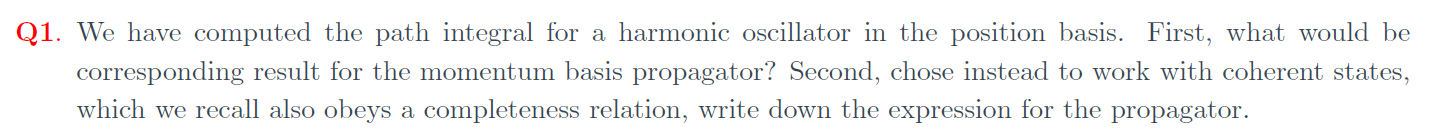
\includegraphics[width=8cm]{1.PNG}
\end{figure}
\end{frame}

\begin{frame}
	\frametitle{Recap of complex analysis so far}
	\begin{block}{Functions of one complex variable}
	Requiring $f$ to be holomorphic in a neighborhood around $z_0$ put great constraints on our functions, i.e. Cauchy Riemann conditions (among others) with $\omega=u+iv$, $z=x+iy$
	\begin{equation}
		\begin{aligned}
			\partial_x u= \partial_y v,~~~~\partial_x v= -\partial_y u
		\end{aligned}
	\end{equation}
	\end{block}
\end{frame}

\begin{frame}
	\frametitle{Some definitions}
	\begin{block}{Some definitions}
	\begin{itemize}
		\item \textbf{Isomorphism}: Structure-preserving mapping between two structures of the same type that can be reversed by an inverse mapping.
		\item \textbf{Homeomorphism}: Isomorphism in the category of topological spaces. I.e. they are the mappings that preserve all the topological properties of a given space
		\item  \text{Injective holomorphic map} is a holomorphic isomorphism
	\end{itemize}
Given a holomorphic injective map from an open set $U$ to $\mathds{C}$
\begin{equation}
	\begin{aligned}
		f:U \to \mathds{C}
	\end{aligned}
\end{equation}
then $f(u)$ is open, and the inverse map is also holomorphic.
	\end{block}
\end{frame}

\begin{frame}
	\frametitle{Complex analysis on surfaces}
	\begin{block}{Complex analysis on surface}
		\begin{itemize}
			\item Take a known surface that we can visualize.
			\item Pick some point $x_0$ on the surface on some disc-like domain $\mathcal{D}$.
			\item Introduce function $f$ that takes on complex values on $\mathcal{D}$.
			\item Extend definition of holomorphic function at $x_0$ so that we can use tools of complex analysis on the surface.
		\end{itemize}
	\end{block}
\begin{figure}
	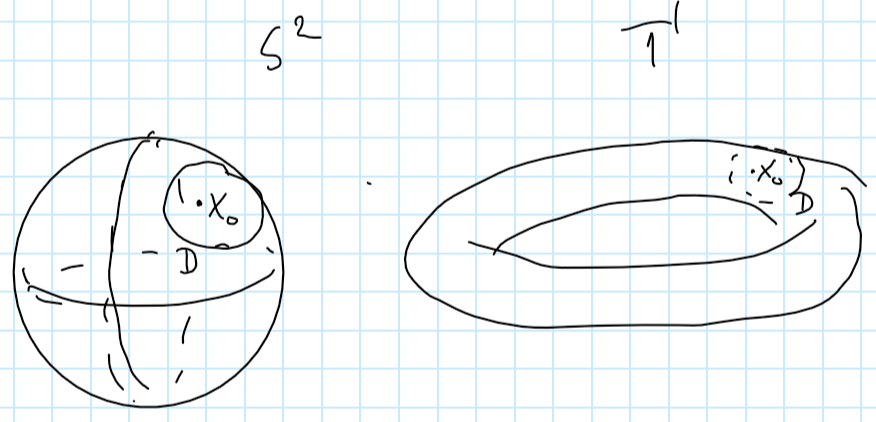
\includegraphics[width=10cm]{2.PNG}
\end{figure}
\end{frame}

\begin{frame}
	\frametitle{Complex analysis on surfaces}
	\begin{block}{Complex analysis on surface}
			Do this by identifying $\mathcal{D}$ with an open subset, say
			\begin{equation}
				\begin{aligned}
					\Delta = \{z\in \mathds{C}~\big|~|z|=1\}
				\end{aligned}
			\end{equation}
		by choosing a homeomorphism 
		\begin{equation}
			\begin{aligned}
				\phi:\mathcal{D}\to \Delta
			\end{aligned}
		\end{equation}
	Hence we now have a map from the unit disc on the surface to the complex plane
\begin{figure}\vspace*{-0.3cm}
	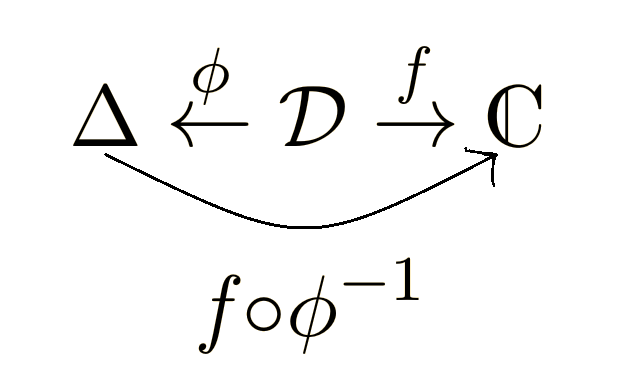
\includegraphics[width=2.7cm]{3}
\end{figure}
	\end{block}
\end{frame}

\begin{frame}
	\frametitle{Complex analysis on surfaces}
	\begin{block}{Complex analysis on surface}
	Require that $f\circ \phi^{-1}$ is holomorphic in points $x$ ind $\mathcal{D}$.
	
	Just like on slide 5, we can say that $f$ is holomorphic on $D$ if $f\circ \phi^{-1}$ is holomorphic on $\Delta$. 
	
	\end{block}
\end{frame}

\begin{frame}
	\frametitle{Complex analysis on surfaces}
	\begin{block}{Complex analysis on surface}
	The pair $(\mathcal{D},\phi)$ is called a \textit{complex coordinate chart}
	
	It allows us to do complex analysis on the disc, but we could have taken any open set.
	\end{block}
\end{frame}

\begin{frame}
	\frametitle{Complex analysis on surfaces}
	\begin{block}{Complex analysis on surface}
		More generally: a complex coorddinate chart is a pair
		\begin{equation}
			\begin{aligned}
				(\mathcal{U},\phi)
			\end{aligned}
		\end{equation}
	where $\mathcal{U}$ is an open subset of $X$ and $\phi:\mathcal{U}\to \mathcal{V}$ is a homemorphism onto an open subset $\mathcal{V}$ of $\mathds{C}$.
	\end{block}
\end{frame}

\section{Applications}
\begin{frame}
	\frametitle{Applications}
	\begin{block}{QFT scattering}
		Overlap between two asymptotic states
		\begin{equation}\label{ScatteringMatrix}
		\braket{f|i}=(2\pi)^D\delta^D\left(\sum_ik_i\right)(\mathds{1}_{fi}+iT_{fi}),
		\end{equation}
		Scattering cross section proportional to $|T_{fi}|^2$.
		
		We refer to $ T_{fi} $ as the scattering amplitude and denote it by $ \mathcal{A}(...) $ where $ (...) $ is the scattering data.
	\end{block}
\end{frame}


\section{The Scattering Equations}
\begin{frame}
	\frametitle{The CHY formalism}
	\begin{block}{Scattering equations and amplitudes}
		The \emph{scattering equations} are given by
		\begin{equation}
		\mathcal{S}_i=\sum_{j\neq i}\frac{s_{ij}}{z_i-z_j}=0,\quad i\in\{1,2,..,n\}.	\label{ScatteringEquations}
		\end{equation}
		One can obtain amplitudes of various theories from the formula
		\begin{equation}
		\mathcal{A}_n(1,...,n)=\int d\Omega_{\text{CHY}} \mathcal{I}(z_i,k_i,\epsilon_i,...), \label{CHYformula1}
		\end{equation}
		with $ d\Omega_{\text{CHY}}=\frac{d^nz}{\text{Vol}(\text{SL}(2,\mathbb{C}))}\prod_{i}'\delta(\mathcal{S}_i) $.
	\end{block}
\end{frame}

\begin{frame}
	\frametitle{Integration rules}
	\begin{block}{Graphic representation of M\"obious invariant integrands}
		We represent the integrands by four-regular graphs. Every factor of $ z_{ij}^{-1} $ is a line between vertices $ i $ and $ j $ and every factor $ z_{ij} $ is a dashed line. 
		\begin{equation}
			\begin{aligned}
				A_3^{\text{YM}}(1,2,3)&=\PT(1,2,3)\Pf' \Psi^{1,3}\\
				&=\frac{1}{z_{12}^2z_{23}^2z_{13}^2}\left\{-\epsilon_{12}\epsilon k_{32}+\epsilon_{13}\epsilon k_{23}+\epsilon_{23}\epsilon k_{12}\right\}\\
				&=\begin{chy}[3]
					\chydoubleline{1}{2};
					\chydoubleline{1}{3};
					\chydoubleline{3}{2};
				\end{chy}\left\{-\epsilon_{12}\epsilon k_{32}+\epsilon_{13}\epsilon k_{23}+\epsilon_{23}\epsilon k_{12}\right\}
				\\
				&=-\epsilon_{12}\epsilon k_{32}-\epsilon_{13}\epsilon k_{21}+\epsilon_{23}\epsilon k_{12}
				, \end{aligned}
		\end{equation}
	\end{block}
\end{frame}


\begin{frame}
	\centering
	\Large Thank you for your attention.\\
\end{frame}		
\end{document}
